\documentclass{article}
\usepackage[utf8x]{inputenc}
\usepackage{ucs}
\usepackage{amsmath} 
\usepackage{amsfonts}
\usepackage{upgreek}
\usepackage[english,russian]{babel}
\usepackage{graphicx}
\usepackage{float}
\usepackage{textcomp}
\usepackage{hyperref}
\usepackage{mathtools}
\usepackage{geometry}
  \geometry{left=2cm}
  \geometry{right=1.5cm}
  \geometry{top=1cm}
  \geometry{bottom=2cm}
\usepackage{tikz}
\usepackage{ccaption}
\usepackage{multicol}
%\setlength{\columnsep}{1.5cm}
%\setlength{\columnseprule}{0.2pt}
\usepackage{listings}

\DeclarePairedDelimiter\ceil{\lceil}{\rceil}
\DeclarePairedDelimiter\floor{\lfloor}{\rfloor}

\begin{document}
\pagenumbering{gobble}

\lstset{
  language=C,                % choose the language of the code
  basicstyle=\linespread{1.1}\ttfamily,
  columns=fixed,
  fontadjust=true,
  basewidth=0.5em,
  keywordstyle=\color{blue}\bfseries,
  commentstyle=\color{gray},
  stringstyle=\ttfamily\color{orange!50!black},
  showstringspaces=false,
  %numbers=false,                   % where to put the line-numbers
  numbersep=5pt,
  numberstyle=\tiny\color{black},
  numberfirstline=true,
  stepnumber=1,                   % the step between two line-numbers.        
  numbersep=10pt,                  % how far the line-numbers are from the code
  backgroundcolor=\color{white},  % choose the background color. You must add \usepackage{color}
  showstringspaces=false,         % underline spaces within strings
  captionpos=b,                   % sets the caption-position to bottom
  breaklines=true,                % sets automatic line breaking
  breakatwhitespace=true,         % sets if automatic breaks should only happen at whitespace
  xleftmargin=.2in,
  extendedchars=\true,
  keepspaces = true,
}
\lstset{literate=%
   *{0}{{{\color{red!20!violet}0}}}1
    {1}{{{\color{red!20!violet}1}}}1
    {2}{{{\color{red!20!violet}2}}}1
    {3}{{{\color{red!20!violet}3}}}1
    {4}{{{\color{red!20!violet}4}}}1
    {5}{{{\color{red!20!violet}5}}}1
    {6}{{{\color{red!20!violet}6}}}1
    {7}{{{\color{red!20!violet}7}}}1
    {8}{{{\color{red!20!violet}8}}}1
    {9}{{{\color{red!20!violet}9}}}1
}

\title{Семинар \#14: Безопасность.\vspace{-5ex}}\date{}\maketitle

\subsection*{Проверка на ошибки. Переменная \texttt{errno} и функция \texttt{perror}.}
\begin{lstlisting}
#include <stdio.h>
int main()
{
	FILE* file = fopen("input.txt", "r");
	if (file == NULL)
	{
		perror("Error");
		exit(1);
	}
	// Работаем с файлом file
}
\end{lstlisting}


\subsection*{Опасность функций семейства \texttt{scanf} при считывании строк.}
Функции \texttt{scanf}, \texttt{fscanf} и \texttt{sscanf} имеют одну неприятную особеность при считывании строк. Спецификатор \texttt{\%s} делает следующее: считывает строку и записывает её всю по передаваемому ей адресу. Это может привести к серьёзным ошибкам если то место, куда мы записываем строку будет меньше, чем записываемая строка. Рассмотрим, например, следующую простую программу:
\begin{lstlisting}
#include <stdio.h>
int main()
{
	char a[5] = "Lion";
	char b[5];

	scanf("%s", b);
	
	printf("a = %s\n", a);
	printf("b = %s\n", b);
}
\end{lstlisting}
\begin{itemize}
\item Что напечатает эта программа, если на вход передать строку \texttt{Cat}?
\item Что напечатает эта программа, если на вход передать строку \texttt{Zebra}?
\item Что напечатает эта программа, если на вход передать строку \texttt{Elephant}?
\item Как исправить ошибки?
\end{itemize}

\begin{center}
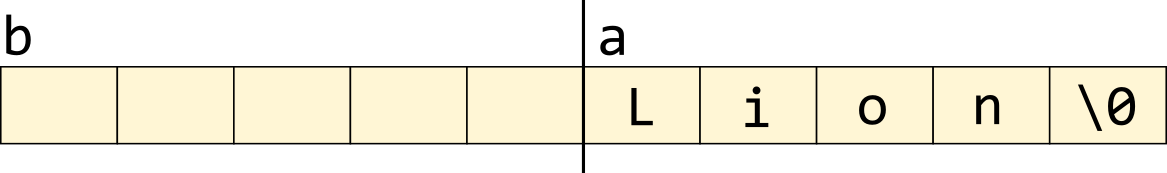
\includegraphics[scale=1]{../images/scanf_safety.png}
\end{center}

Функция \texttt{scanf} выходит за границы массива \texttt{b} и переписывает другую строку. Если бы на месте строки \texttt{a} была бы переменная другого типа, то \texttt{scanf} испортил бы и её. Более того, таким поведением \texttt{scanf} могут воспользоваться

\subsection*{Функции \texttt{ftell} и \texttt{fseek}}

\end{document}
